\section{Obstructed P-nodes} \label{sec:p_nodes}

If a P-node is obstructed, then it has some subtrees $T_1,\dots,T_n$ forming the cycle $T_1 \wlt T_2
\wlt \cdots \wlt T_n \wlt T_1$.  We start by showing that the specific structure of $\wlt$ forces
the existence of a two-cycle, so we can assume that $n=2$.

\begin{lemma} \label{lem:p_node_two_cycle}
If a P-node is obstructed, then it has two subtrees $T_1$ and $T_2$ such that $T_1 \wlt T_2 \wlt
T_1$.
\end{lemma}

\begin{figure}[b!]
\centering
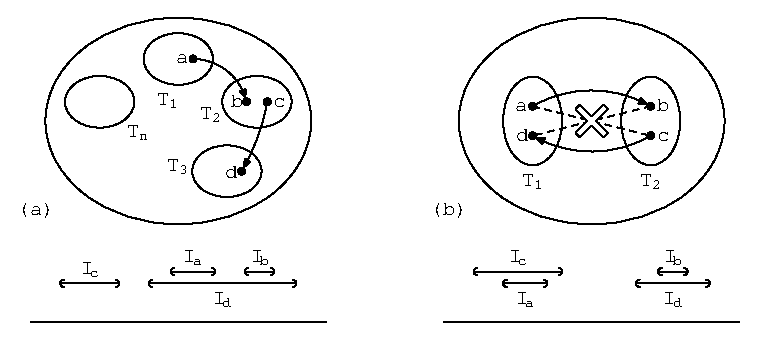
\includegraphics{p_nodes_cycles.eps}
\caption{(a) At the top, a shortest $n$-cycle of $\wlt$ on the children of a P-node. At the bottom, the
derived positions of the open intervals. (b) At the top, the four cliques involved in a two-cycle in $\wlt$.
The cliques $a$ and $c$ are incomparable, and so are $b$ and $d$. At the bottom, one of the four
possible configurations of the open intervals.}
\label{fig:P_node_cycles}
\end{figure}

\begin{proof}
The proof is illustrated in Fig.~\ref{fig:P_node_cycles}a.  Let $T_1 \wlt \cdots \wlt T_n \wlt T_1$
be a shortest cycle for the obstructed P-node. To get a contradiction, we assume $n \ge 3$. Since
$T_1 \wlt T_2$, there exist $a \in T_1$ and $b \in T_2$ such that $a \wlt b$.  Similarly, there
exist $c \in T_2$ and $d \in T_3$ such that $c \wlt d$.  We know that $I_a$ is on the left of $I_b$,
and $I_c$ is on the left of $I_d$. We analyze the remaining relative positions.

First, $I_d$ is not on the right of $I_a$, since otherwise $T_1 \wlt T_3$ and a shorter cycle would
exist. Additionally, $I_d$ is not on the left of $I_b$, since we would get $T_3 \wlt T_2$, and $T_2$
and $T_3$ would form a two-cycle. According to Lemma~\ref{lem:single_overlap}, no single overlaps of
open intervals are allowed, so $I_d$ necessarily contains both $I_a$ and $I_b$; see
Fig.~\ref{fig:P_node_cycles}a. Therefore, $I_c$ is on the left of $I_a$, so $T_2 \wlt T_1$ and we
get a two-cycle.\qed
\end{proof}

To create a two-cycle, at most four cliques are enough.  Aside from Lemma~\ref{lem:single_overlap},
so far we have not used that $\wlt$ arises from a partial interval representation. Next, we use
properties of the MPQ-tree.

\begin{lemma} \label{lem:p_node_three_cliques}
A two-cycle $T_1 \wlt T_2 \wlt T_1$ is created by at most three cliques.
\end{lemma}

\begin{proof}
The proof is depicted in Fig.~\ref{fig:P_node_cycles}b. Suppose that this two-cycle is given by four
cliques $a,d \in T_1$ and $b,c \in T_2$ such that $a \wlt b$ and $c \wlt d$. Assume for
contradiction that no three of these cliques define the two-cycle, i.e., $a$ and $c$ are
incomparable, and so are $b$ and $d$. According to Lemma~\ref{lem:single_overlap}, $I_a \subseteq
I_c$ or $I_a \supseteq I_c$, and analogously for $I_b$ and $I_d$. In all of the four cases, $I_c$ is
on the left of $I_b$, and $I_d$ is on the right of $I_a$.

We look at the case where $I_a \subseteq I_c$ and $I_b \subseteq I_d$, as in
Fig.~\ref{fig:P_node_cycles}b. By Lemma~\ref{lem:open_intervals}, we have $P(c) \subseteq P(a)$.
Therefore, $P(c)$ contains no vertices from the sections of $T_2$. Similarly, $P(d) \subseteq P(b)$,
and $P(d)$ contains no vertices from the sections of $T_1$. Therefore $P(c) = P(d)$, which implies
$I_c = I_d$, a contradiction. The other cases can be analyzed similarly.\qed
\end{proof}

It remains to put these results together and characterize the possible obstructions.

\begin{lemma}[The P-node case] \label{lem:p_node}
If a P-node is obstructed, then $G$ and $\calR'$ contain an SE, $1$-FAT, or $1$-BI obstruction.
\end{lemma}

\begin{proof}
According to Lemma~\ref{lem:p_node_two_cycle}, the obstructed P-node has a two-cycle in $\wlt$.  By
Lemma~\ref{lem:p_node_three_cliques}, there are at most three maximal cliques defining this cycle.  First
assume that this cycle is defined by two cliques $a \in T_1, b \in T_2$ such that $a \wlt b \wlt a$.
According to the definition of $\wlt$, this implies that $I_a = I_b$, both of lenght zero.
Therefore $P(a) = P(b)$. Let $u \in P^{\endlft}(a)$ and $v \in P^{\startrt}(a)$ (possibly $u=v$); we
have that $\inter u' \cap \inter v'$ is a singleton.  Since $a$ and $b$ are two maximal cliques,
there exists $x \in a \setminus b$ and $y \in b \setminus a$. We get an SE obstruction.

It remains to deal with the case where three cliques define the two-cycle. Let $a,c \in T_1$ and $b
\in T_2$ such that $a \wlt b \wlt c$. We have three non-intersecting intervals whose left-to-right
order is $I_a$, $I_b$ and $I_c$. Since $I_a$ and $I_c$ are disjoint, one of the sets $P(a) \setminus
P(c)$ and $P(c) \setminus P(a)$ is non-empty. Without loss of generality, we assume that $P(a)
\setminus P(c)\neq \emptyset$. Let $p \in P(a) \setminus P(c)$; then $p$ belongs to sections of
$T_1$, and as a consequence $p \notin P(b)$. Therefore $\inter p'$ is on the left of $I_b$.  We
distinguish two cases.

\begin{figure}[b!]
\centering
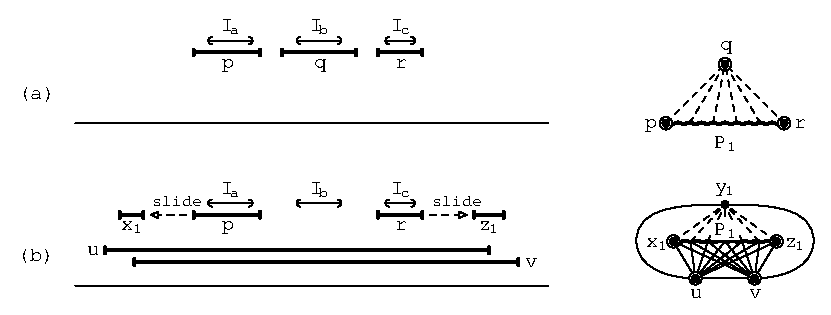
\includegraphics{p_nodes_two_cases.eps}
\caption{The two cases of the proof of Lemma~\ref{lem:p_node}. (a) Case 1 leads to a 1-FAT
obstruction. (b) Case 2 leads to a 1-BI obstruction.}
\label{fig:P_node_two_cases}
\end{figure}

\emph{Case 1:} $P(b) \setminus P(c) \ne \emptyset$. We choose $q \in P(b) \setminus P(c)$. Then
$q$ belongs to sections of $T_2$, and $\inter q'$ is between $\inter p'$ and $I_c$. In
the next paragraph we show that there also exists $r \in P(c) \setminus P(b)$. Then $r$ belongs to sections of
$T_1$, and $\inter r'$ is on the right of $\inter q'$, as in Fig.~\ref{fig:P_node_two_cases}a. By
Lemma~\ref{lem:connectivness}(ii), $G[T_1]$ is connected; let $P_1$ be a shortest
path from $p$ to $r$ in $G[T_1]$. We obtain a $1$-FAT obstruction for $x_1 = p$, $y_1 = q$ and $z_1 = r$.

It remains to show that such $r$ exists. Suppose for contradiction that $P(c) \setminus P(b)
= \emptyset$. Since $P(c) \subsetneq P(b)$, no vertex of $P(c)$ appears in sections of $T_1$,
and we get $P(c) \subsetneq P(a)$. Consequently, every pre-drawn interval of $P(c)$ contains
$[\clql(a),\clqr(c)]$. The position of $I_c$ implies that every point of $[\clql(a),\clql(c))$ is
covered by some pre-drawn interval not contained in $P(c)$. In particular, there exists a path from
$p$ to $q$ consisting of such intervals. Since $p$ belongs to
sections of $T_1$ and $q$ belongs to sections of $T_2$, every path from $p$ to $q$ 
contains a vertex of the section of the P-node, or of a section above it; hence, the path contains a
vertex belonging to $c$. We obtain a contradiction.

\emph{Case 2:} $P(b) \setminus P(c) = \emptyset$. Then there exists $r \in P(c) \setminus P(b)$. 
We again observe that $\inter r'$ is on the right of $I_b$, as depicted in
Fig.~\ref{fig:P_node_two_cases}b. Furthermore, $P(b) \subseteq P(a) \cap P(c)$, so every
pre-drawn interval of $P(b)$ contains $[\clql(a),\clqr(c)]$.

We construct a 1-BI obstruction and we name the vertices as in the definition. Let $u \in
P^\endlft(b)$ and $v \in P^\startrt(b)$ (possibly $u = v$). Since $p$ does not necessarily cover
$\ell(v)$ and $r$ does not necessarily cover $r(u)$, we might not be able to construct a $1$-BI
obstruction with $x_1=p$ and $z_1=q$. We instead use Sliding Lemma~\ref{lem:sliding}. By applying it
(flipped) to $I_b$, $I_a$ and $p$, we obtain a pre-drawn interval $x_1$ covering $\ell(v)$ (possibly
$x_1 = p$). By applying it to $I_b$, $I_c$ and $r$, we obtain a pre-drawn interval $z_1$ covering
$r(u)$ (possibly $z_1 = r$). Furthermore, $x_1$ and $z_1$ belong to sections of $T_1$. Since
$G[T_1]$ is connected by Lemma~\ref{lem:connectivness}(ii), there exists a shortest path $P_1$ from
$x_1$ to $z_1$ containing no vertex of $b$. By Lemma~\ref{lem:non_adjacent}, there exists $y_1 \in
b$ non-adjacent to all vertices of $P_1$. We obtain a $1$-BI obstruction.\qed
\end{proof}

